\documentclass{article}
\usepackage{realtristan}
\title{Physics Dynamics + Motion}
\author{Tristan Simpson}
\begin{document}
\maketitle
\tableofcontents

\section{Equations}

\section{Units}

\section{Kinematics}

\section{Forces}

\section{Incline Planes}

\section{Elevators}

\section{Notes}
\begin{itemize}
    \item All Forces of Tension ($F_T$) are equal. Example: $F_{T_1} = F_{T_2} = F_{T_3}$
\end{itemize}

\section{Pulleys}
\subsection{Pulleys Example Problem 1}
An atwood machine consists of masses of 3.8 kg and 4.2 kg. What is the acceleration ($a$) of the masses? What is the tension ($F_T$) in the rope?
\subsubsection{Diagram and Givens}
\flex{}{
    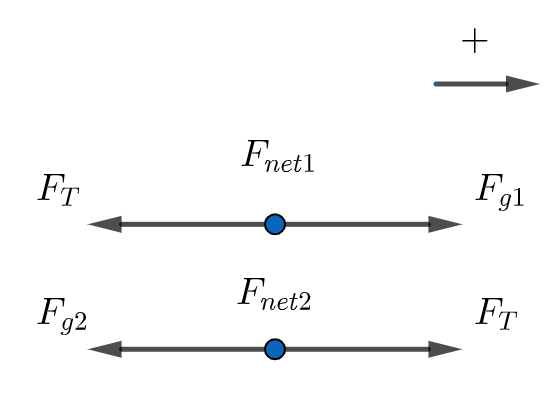
\includegraphics[scale=0.5]{images/pulleys_diagram_1}
}
\flex{}{
    \begin{itemize}
        \item $m_1 = 3.8\;\text{kg}$
        \item $m_2 = 4.2\;\text{kg}$
        \item $g = 9.8\;\text{m}/\text{s}^2$
        \item $a =\;?$
        \item $F_T =\;?$
    \end{itemize}
}

\subsubsection{Finding equation for $F_T$}
\begin{flalign*}
     & \therefore\;\;F_{net_2} = F_T - F_{g_2}                              \\\\
     & \hookrightarrow\;\;m_2a = F_T - m_2g\;\;\;\to\;\;\;m_2a + m_2g = F_T \\\\
     & \therefore\;\;F_T = m_2a + m_2g                                      \\
\end{flalign*}\leavevmode

\subsubsection{Finding equation for $a$}
\begin{flalign*}
     & \therefore\;\; F_{net_1} = F_{g_1} - F_T                                             \\\\
     & \hookrightarrow\;\;m_1a = m_1g - F_T\;\;\;\to\;\;\;m_1a = m_1g - (m_2a + m_2g)       \\\\
     & \hookrightarrow\;\;m_1a = m_1g - m_2a - m_2g\;\;\;\to\;\;\;m_1a + m_2a = m_1g - m_2g \\\\
     & \hookrightarrow\;\;a(m_1 + m_2) = g(m_1 - m_2)                                       \\\\
     & \therefore\;\;a = \left(\frac{g(m_1 - m_2)}{(m_1 + m_2)}\right)                      \\
\end{flalign*}\leavevmode

\subsubsection{Solving for $a$}
\begin{flalign*}
    \therefore\;\;a & = \left(\frac{9.81(4.2 - 3.8)}{(4.2 + 3.8)}\right)\;\approx\; 0.49\;\text{m}/\text{s}^2 \\
\end{flalign*}\leavevmode


\subsubsection{Solving for $F_T$}
\begin{flalign*}
    \therefore\;\;F_T & = m_2a + m_2g                                  \\\\
                      & = 3.8(0.49) + 3.8(9.81)\;\approx\;39\;\text{N}
\end{flalign*}\leavevmode\\

\subsection{Pulleys Example Problem 2}
The smaller mass on an Atwood machine is 5.2kg. If the masses accelerate at 4.6 m/$s^2$, what is the mass of the larger object? What is the tension in the rope?

\subsubsection{Diagram and Givens}
\flex{}{
    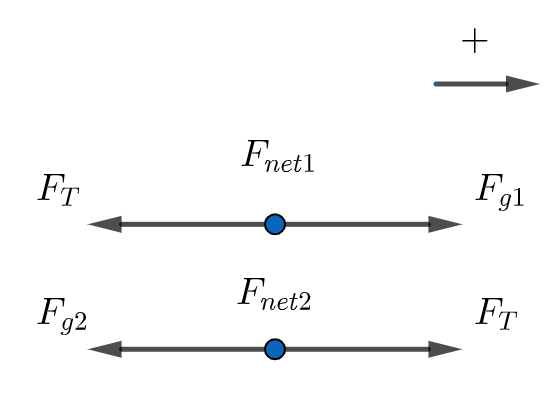
\includegraphics[scale=0.5]{images/pulleys_diagram_1}
}
\flex{}{
    \begin{itemize}
        \item $m_2 = 5.2\;\text{kg}$
        \item $m_1 = \;?$
        \item $g = 9.8\;\text{m}/\text{s}^2$
        \item $a = 4.6\;\text{m}/\text{s}^2$
        \item $F_T =\;?$
    \end{itemize}
}
\subsubsection{Solving for $m_1$}


\section{Projectile Motion 1}

\section{Projectile Motion 2}

\section{Newton's Laws}

\section{Labs}

\section{Theory}


\end{document}